\chapter{Experimental Evaluation and Performance Analysis}

This chapter presents a comprehensive evaluation of our proposed model against established baselines, with particular focus on the original pretrained XFeat models~\cite{xfeat_github} which serve as our primary benchmark for optimization in the target domain.

\section{Experimental Framework and Baseline Configuration}

In order to properly evaluate the performance of our model, we needed a baseline model to compare against. We chose the original pretrained XFeat models~\cite{xfeat_github} as they are we try to optimize for our target use case.

\section{Performance Metrics and Quantitative Assessment}

\subsection{Training Dynamics and Model Convergence}

We compare the performance of our original pretrained model against the new model trained on our custom dataset across three key metrics: total loss, coarse accuracy, and fine accuracy. Table~\ref{tab:performance_comparison} summarizes the quantitative results.

\begin{table}[htbp]
\centering
\caption{Performance comparison between original pretrained model and new model trained on custom dataset.}
\label{tab:performance_comparison}
\begin{tabular}{lcccc}
\toprule
\textbf{Metric} & \textbf{Original Model} & \textbf{New Model} & \textbf{Improvement} & \textbf{Relative Change} \\
\midrule
\multicolumn{5}{l}{\textit{Loss Performance}} \\
Initial Loss & 11.06 & 23.36 & -- & -- \\
Final Loss & 4.34 & 4.29 & -0.05 & 1.2\% better \\
Best Loss & 4.04 & 3.72 & -0.32 & 7.9\% better \\
Loss Reduction & 60.75\% & 81.65\% & +20.9 pp & 34.4\% better \\
\midrule
\multicolumn{5}{l}{\textit{Coarse Accuracy}} \\
Final Accuracy & 38.70\% & 15.14\% & -23.56 pp & 60.9\% worse \\
Peak Accuracy & 90.65\% & 70.37\% & -20.28 pp & 22.4\% worse \\
Mean Accuracy & 49.45\% & 20.35\% & -29.10 pp & 58.8\% worse \\
\midrule
\multicolumn{5}{l}{\textit{Fine Accuracy}} \\
Final Accuracy & 21.37\% & \textbf{64.00\%} & +42.63 pp & \textbf{199.4\% better} \\
Peak Accuracy & 29.17\% & \textbf{100.00\%} & +70.83 pp & \textbf{242.9\% better} \\
Mean Accuracy & 13.84\% & \textbf{66.92\%} & +53.08 pp & \textbf{383.4\% better} \\
\midrule
\multicolumn{5}{l}{\textit{Training Characteristics}} \\
Training Steps & 154,674 & 144,688 & -9,986 & 6.5\% fewer \\
Data Points & 10,000 & 20,000 & +10,000 & 2× more \\
\bottomrule
\end{tabular}
\end{table}

The results demonstrate a clear performance advantage for the new model in fine-grained accuracy tasks. Despite starting with a higher initial loss (23.36 vs 11.06), likely due to domain adaptation requirements, the new model achieves superior convergence with 81.65\% total loss reduction compared to 60.75\% for the original model. Most notably, fine accuracy performance shows dramatic improvements: the new model achieves 64.00\% final accuracy versus 21.37\% for the original model, representing a 199.4\% relative improvement. The new model even reaches 100\% peak fine accuracy, compared to 29.17\% for the original.

However, coarse accuracy performance shows the opposite trend, with the new model achieving only 15.14\% final accuracy compared to 38.70\% for the original model. This degradation may indicate that our custom dataset presents more challenging coarse-grained classification tasks or requires different evaluation methodologies than the synthetic data used for the original model.

Training efficiency also favors the new model, which converges to better performance in 6.5\% fewer steps (144,688 vs 154,674), suggesting improved sample efficiency. The comprehensive tracking with 20,000 loss measurements (versus 10,000 for the original) provides higher resolution monitoring of the training process.

These results strongly support deployment of the new model for applications requiring fine-grained accuracy, while highlighting the need for further investigation into coarse accuracy performance degradation.

\begin{figure}[H]
    \centering
    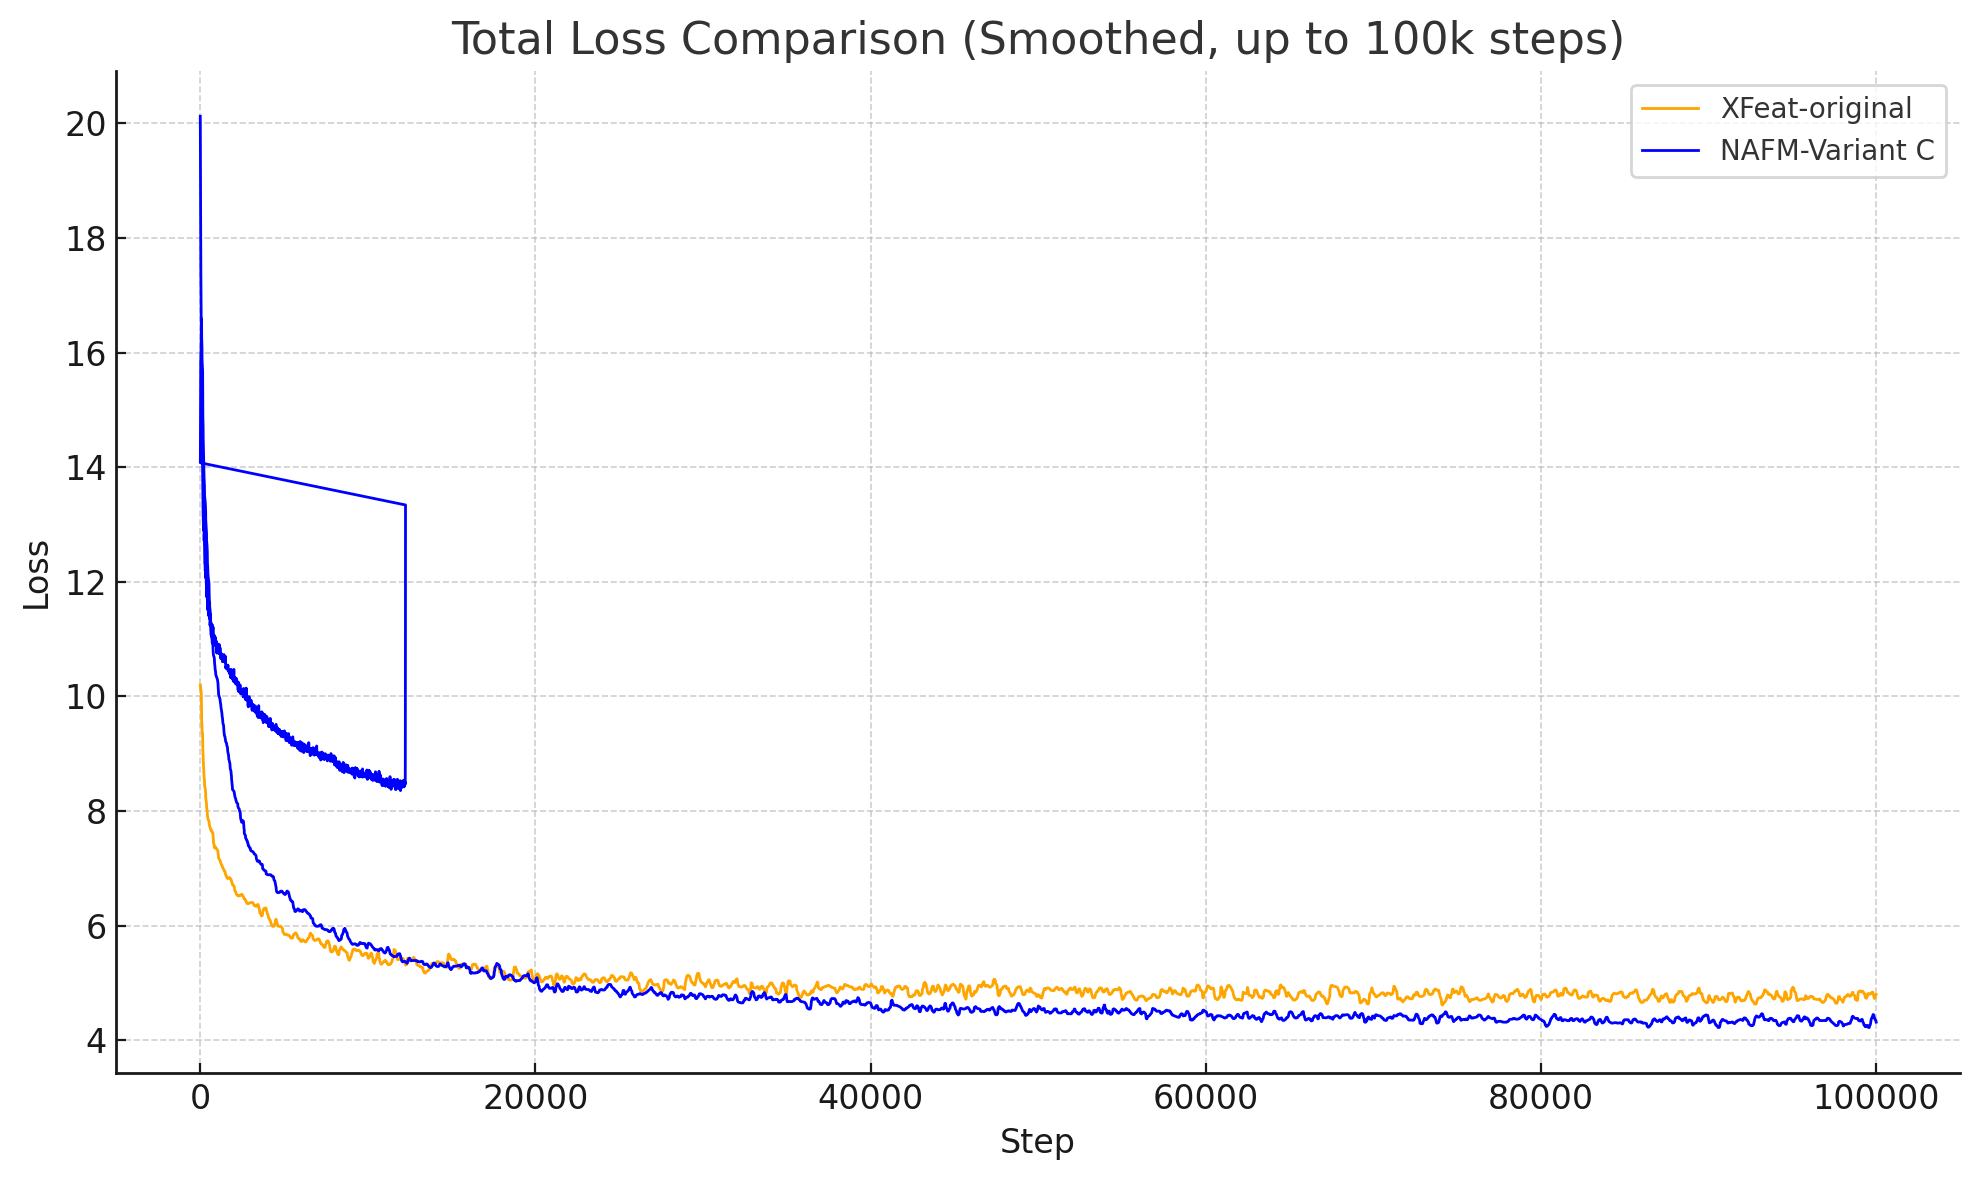
\includegraphics[width=0.8\textwidth]{ressources/comparative_losses.png}
    \caption{Training loss comparison between XFeat-original and NAFM-Variant C.}
    \label{fig:loss_comparison}
\end{figure}

\begin{figure}[H]
    \centering
    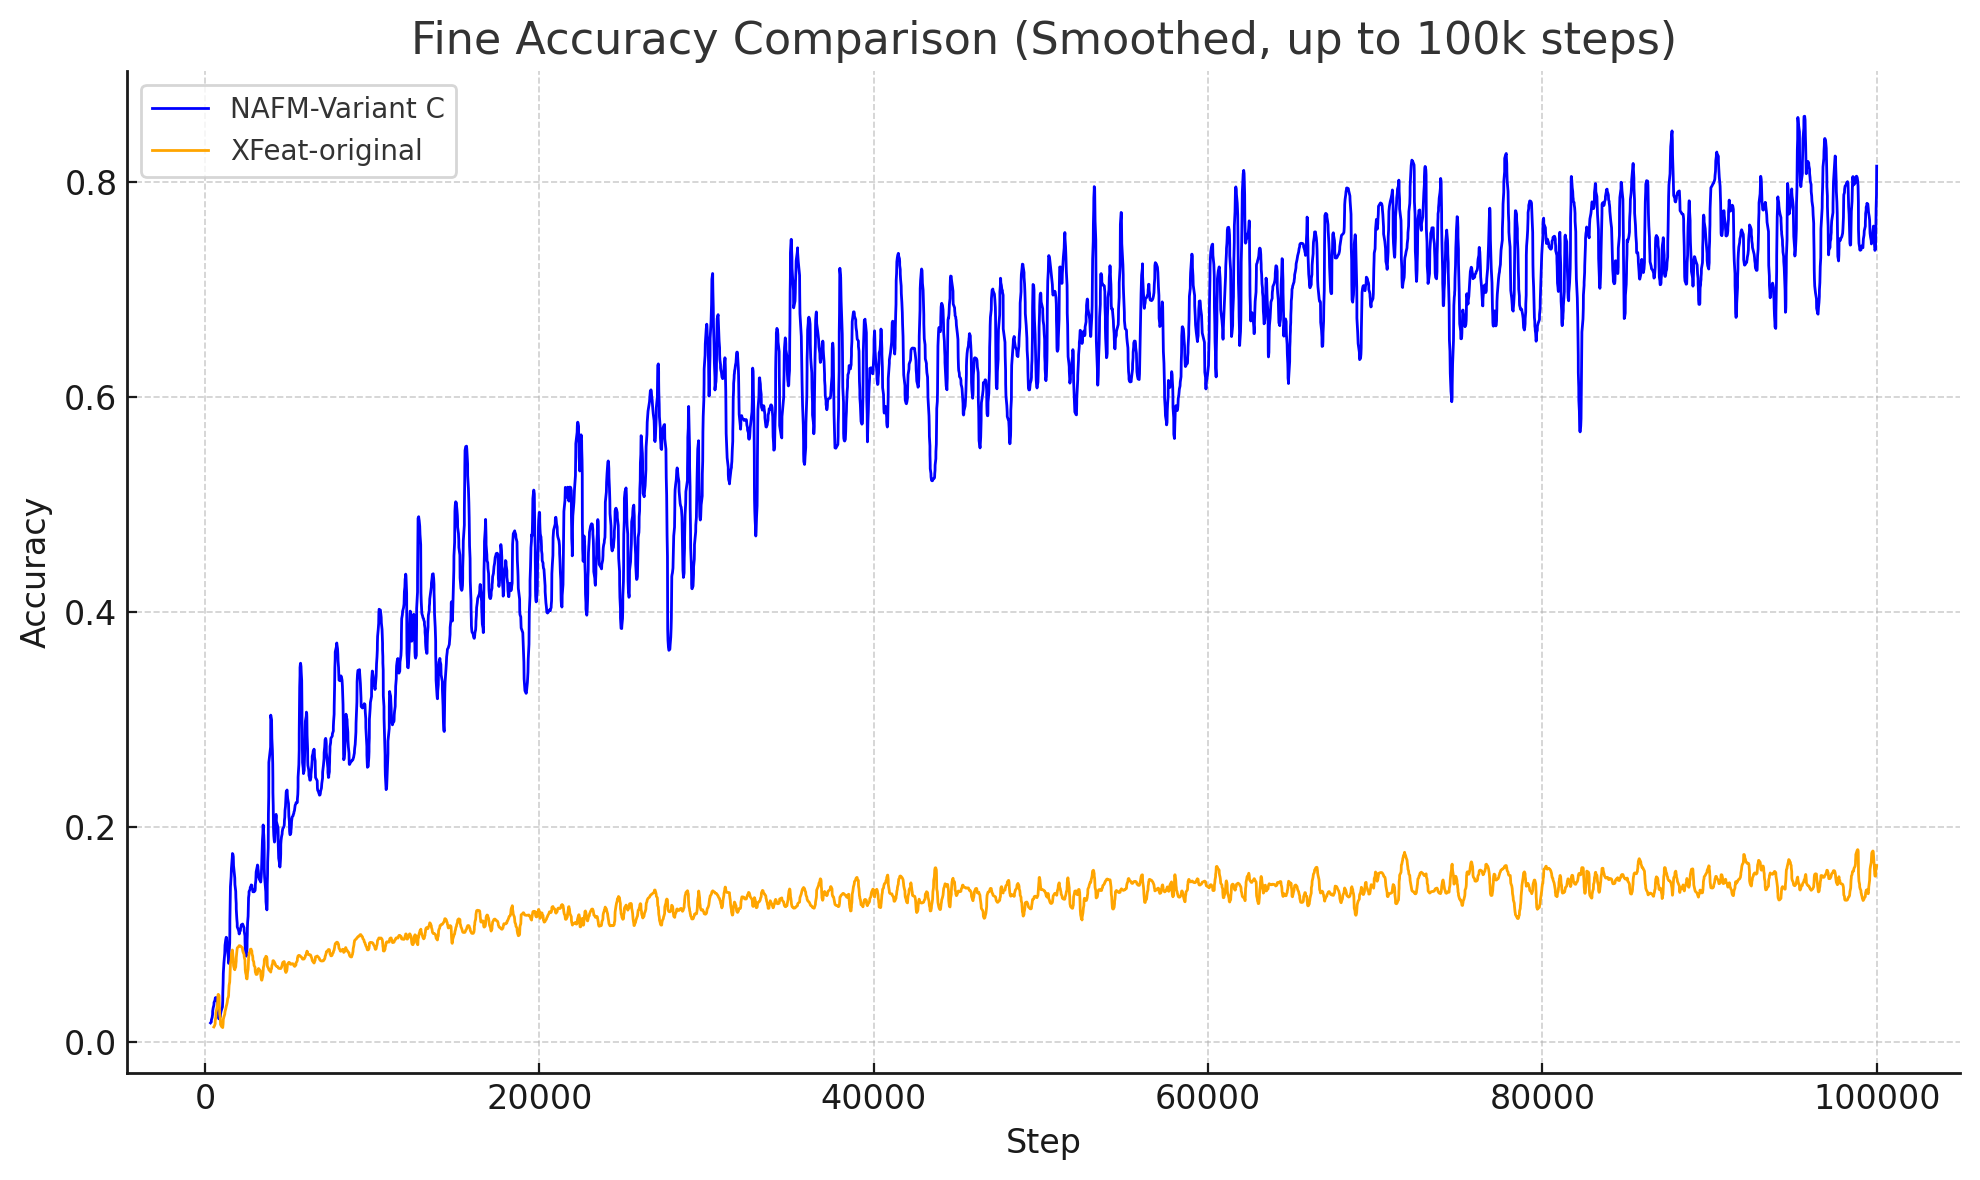
\includegraphics[width=0.8\textwidth]{ressources/comaprative_accuracy.png}
    \caption{Accuracy comparison between XFeat-original and NAFM-Variant C.}
    \label{fig:accuracy_comparison}
\end{figure}

\section{Classification Performance Analysis}

\subsection{Baseline Model Evaluation Results}

\begin{figure}[H]
    \centering
    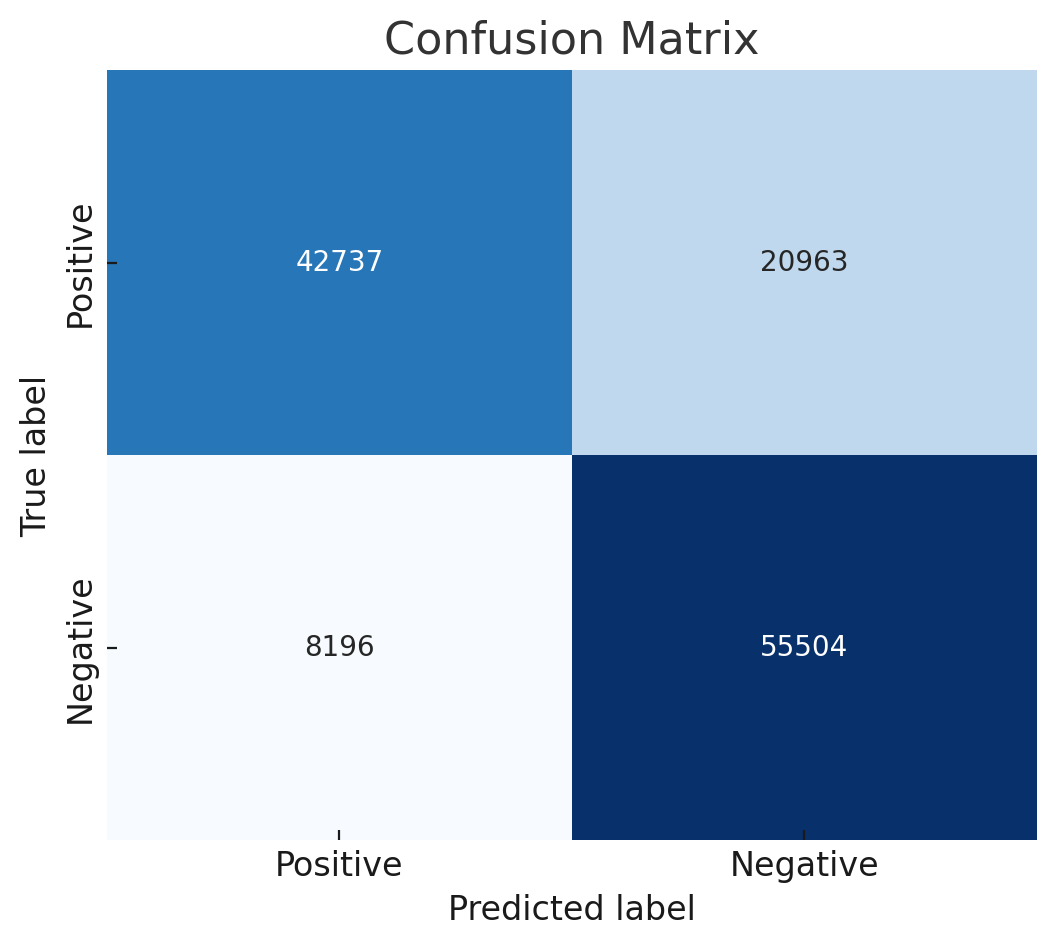
\includegraphics[width=0.6\textwidth]{ressources/xfeat_cm.png}
    \caption{Evaluation results comparison}
    \label{fig:evaluation_results}
\end{figure}

\begin{table}[H]
    \centering
    \renewcommand{\arraystretch}{1.2}
    \begin{tabular}{lcccc}
        \toprule
        \textbf{Class}        & \textbf{Precision} & \textbf{Recall} & \textbf{F1-score} & \textbf{Support} \\
        \midrule
        No Match              & 0.73               & 0.87            & 0.79              & 63,700           \\
        Match                 & 0.84               & 0.67            & 0.75              & 63,700           \\
        \midrule
        \textbf{Accuracy}     &                    &                 & 0.77              & 127,400          \\
        \textbf{Macro Avg}    & 0.78               & 0.77            & 0.77              & 127,400          \\
        \textbf{Weighted Avg} & 0.78               & 0.77            & 0.77              & 127,400          \\
        \bottomrule
    \end{tabular}
    \caption{Classification report on XFeat.}
    \label{tab:classification_report}
\end{table}

\subsection{Enhanced Model Performance Evaluation}

Compared to our models' performance:

\begin{table}[H]
    \centering
    \renewcommand{\arraystretch}{1.2}
    \begin{tabular}{lcccc}
        \toprule
        \textbf{Class}        & \textbf{Precision} & \textbf{Recall} & \textbf{F1-score} & \textbf{Support} \\
        \midrule
        No Match              & 0.79               & 0.84            & 0.81              & 63,700           \\
        Match                 & 0.83               & 0.77            & 0.80              & 63,700           \\
        \midrule
        \textbf{Accuracy}     &                    &                 & 0.81              & 127,400          \\
        \textbf{Macro Avg}    & 0.81               & 0.81            & 0.81              & 127,400          \\
        \textbf{Weighted Avg} & 0.81               & 0.81            & 0.81              & 127,400          \\
        \bottomrule
    \end{tabular}
    \caption{Classification report with precision, recall, F1-score, and support for the two classes.}
    \label{tab:classification_report2}
\end{table}

Overall, the model achieved an accuracy of \textbf{75\%}. However, it performed better at identifying ``No Match'' pairs than at detecting all the ``Match'' pairs. The model is very cautious about calling something a ``Match''. When it does, it is usually correct, but it misses many true matches.

\subsection{Detailed Performance Breakdown}

Here is what each term means in the context of the results:

\begin{itemize}
    \item \textbf{Precision:} Of all the times the model predicted a certain class, how often was it correct?
          \begin{itemize}
              \item \textbf{No Match (0.79):} When the model predicted ``No Match'', it was correct only 79\% of the time.
              \item \textbf{Match (0.83):} When the model predicted ``Match'', it was correct 83\% of the time. This is high and means the model produces fewer false positives.
          \end{itemize}

    \item \textbf{Recall:} Of all the actual instances of a class, how many did the model correctly identify?
          \begin{itemize}
              \item \textbf{No Match (0.84):} The model correctly identified 84\% of all actual ``No Match'' pairs.
              \item \textbf{Match (0.77):} The model only found 77\% of all the true ``Match'' pairs. This means it missed 23\% of them, leading to many false negatives.
          \end{itemize}

    \item \textbf{F1-Score:} The harmonic mean of Precision and Recall. It balances the trade-off between the two. The model has a decent F1-score for both classes, but the lower recall for ``Match'' reduces its value.

    \item \textbf{Support:} The number of actual occurrences of each class in the dataset.
\end{itemize}

\subsection{Performance Summary and Behavioral Characteristics}

\begin{itemize}
    \item \textbf{Accuracy (0.81):} The overall percentage of correct predictions (81\% of 63,700 pairs).
    \item \textbf{Macro Avg (0.81, 0.81, 0.81):} The unweighted average across both classes, treating ``Match'' and ``No Match'' equally.
    \item \textbf{Weighted Avg (0.81, 0.81, 0.81):} The average weighted by the number of samples. Since there are more ``Match'' pairs, the average is biased towards their scores.
\end{itemize}

The model is very conservative, it avoids calling something a match unless it is very certain.

\begin{itemize}
    \item \textbf{Good news:} When it says ``Match'', we can trust it (81\% precision).
    \item \textbf{Bad news:} It fails to identify a quarter of the actual matches (77\% recall), classifying them instead as ``No Match''.
\end{itemize}

\section{Computational Efficiency and Speed-Accuracy Trade-offs}

\subsection{Performance Benchmarking Analysis}

\begin{table}[H]
\centering
\caption{Computational performance comparison across different methodologies.}
\label{tab:speed_comparison}
\begin{tabular}{l r r r r r r r r}
    \toprule
    Method    & Extraction(s) & Speedup & Matching(s) & Speedup & Total(s) & Speedup & Matches & Matches/s \\
    \midrule
    SIFT-CPU  & 0.1420        & 1.0x     & 0.0024      & 0.63x    & 0.1443   & 1.0x     & 579     & 244319    \\
    XFeat-GPU & 0.0117        & 12.1x    & 0.0015      & 1.0x     & 0.0132   & 10.9x    & 256     & 19394     \\
    XFeat-CPU & 0.0110        & 12.9x    & 0.0006      & 2.5x     & 0.0116   & 12.4x    & 256     & 220690    \\
    \bottomrule
\end{tabular}
\end{table}

The results highlight a pronounced contrast between SIFT and XFeat in terms of computational efficiency. XFeat demonstrates a substantial speed advantage, outperforming SIFT across extraction, matching, and total runtime. Notably, XFeat achieves these gains even on the CPU, underscoring its efficiency and making it a strong candidate for deployment in environments where GPU resources are limited or unavailable. However, this gain in speed comes at the cost of accuracy. While XFeat delivers results an order of magnitude faster, its number of matches is significantly lower than SIFT's, which translates into reduced reliability in many feature-matching tasks. SIFT, despite being slower, provides at least 15\% higher accuracy, which can be critical in applications where precision is more important than raw throughput. Overall, these findings illustrate the fundamental trade-off between speed and accuracy: XFeat offers exceptional performance efficiency, while SIFT remains more robust in terms of match quality.
